\scanpage{66}
\diagram{\begin{array}{cc||c|c||cc|cc}
&&&&\multicolumn{2}{c|}{\text{NB de \unsure{pos}}}&\multicolumn{2}{c}{\text{Nb de \unsure{feuillets|feuilles}}}\\
D_5&D_5\times\mathbb Z/2\mathbb Z&\mathbb Z/5\mathbb Z&D_5&12&\deleted{\unsure{6|12}}\inserted{12}&12&6\\[8pt]
\mathbb Z/4\mathbb Z&\begin{gathered}D_4\supset\mathbb Z/2\mathbb Z\\[-3pt]\qquad\times\mathbb Z/2\mathbb Z\end{gathered}&\mathbb Z/2\mathbb Z&\mathbb Z/2\mathbb Z\times\mathbb Z/2\mathbb Z&30&15&30&15\\[8pt]
\deleted{\mathbb Z/\unsure{3}\mathbb Z}&\mathfrak S_3\times\mathbb Z/2\mathbb Z&\mathbb Z/3\mathbb Z&\mathfrak S_3&20&10&20&10
\end{array}}
\figure{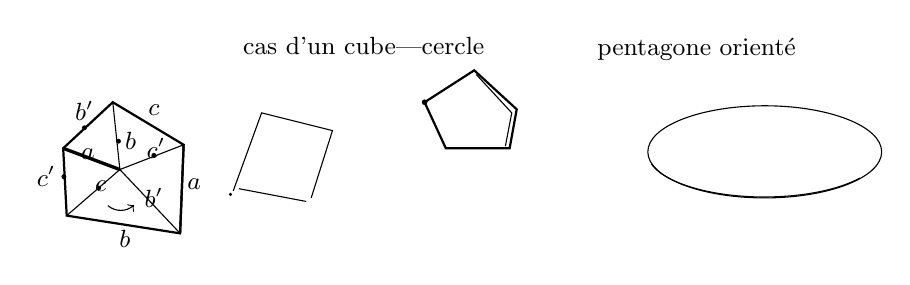
\begin{tikzpicture}[scale=.9,every node/.style={font=\small}]
\node[anchor=west]at(3,2.25){cas d'un \unsure{cube|cercle}};
\node[anchor=west]at(8,2.2){pentagone orienté};
\begin{scope}[shift={(1.4,.6)}]
\draw[thick](-.8,.2)--(-.1,.85)--(.9,.25)--(.85,-1)--(-.75,-.75)--cycle;
\draw[very thick](-.8,.2)--(0,-.1);\draw[thick](.9,.25)--(.85,-1);
\draw(-.1,.85)--(0,-.1)--(.85,-1);\draw(-.75,-.75)--(0,-.1)--(.9,.25);
\foreach\p in{(-.5,.49),(-.79,-.2),(-.02,.3),(-.3,-.36),(.48,.1)}\fill\p circle(.035);
\draw[->](-.17,-.61)to[bend right=40](.2,-.6);
\node at(-.5,.73){$b'$};\node at(.48,.74){$c$};\node at(-.45,.12){$a$};\node at(.15,.3){$b$};\node at(.51,.2){$c'$};\node at(-1.04,-.2){$c'$};\node at(-.27,-.34){$\unsure{c}$};\node at(.48,-.5){$b'$};\node at(1.05,-.3){$a$};\node at(.07,-1.08){$b$};
\end{scope}
\draw[thin](3,.2)--(3.4,1.3)--(4.4,1.05)--(4.1,.1);\draw[thin](3.08,.23)--(4.03,.05);\fill(2.96,.15)circle(.025);
\draw[thick](6,.8)--(5.7,1.45)--(6.4,1.9)--(7,1.35)--(6.9,.8)--cycle;
\draw[thin](6.43,1.84)--(6.93,1.3)--(6.84,.83);\fill(5.7,1.45)circle(.04);
\draw(10.5,.75)ellipse(1.65 and .65);\draw[thin](8.9,.58)arc(195:325:1.65 and .63);
\end{tikzpicture}}

\figure{\begin{tikzpicture}
\node[rotate=180,inner sep=0pt] {\begin{minipage}{13.8cm}\footnotesize
\begin{tabular}{l@{\hspace{1.5cm}}l}
U N I V E R S I T E&MONTPELLIER, le 31 MAI 1979\\
DES SCIENCES ET TECHNIQUES&\\
DU LANGUEDOC&\\
------------&\\
Service de la Scolarité&\\
MR / GJ&\\
Diffusion : Liste A&\\
N\textsuperscript{o} : 3161&
\end{tabular}

\begin{center}
\uline{AVIS DE SOUTENANCE D'UNE THESE DE DOCTORAT D'UNIVERSITE}\\[5pt]
\uline{( SCIENCES\quad NATURELLES )}
\end{center}

\uline{Nom et prénom du candidat} : B E Y R I E S\quad A n d r é

\uline{Titre de la thèse} : Le greffage, moyen de lutte contre les parasites telluriques des Solanées cultivées pour leurs fruits.

\uline{Date, heure et lieu de soutenance prévus:}
\begin{center}20 JUIN 1979 à 10 Heures\\Salle de cours n\textsuperscript{o} 5\end{center}

\uline{Nom du Directeur de thèse} :
\begin{center}Monsieur le Professeur VAGO.\end{center}

\uline{Désignation du laboratoire où la thèse est préparée} :

Laboratoire de Recherches de la Chaire de Biologie et Pathologie Végétales ENSA et INRA - Montpellier .

\uline{Résumé de la thèse} :

\hspace*{2cm}L'objectif de ce travail, commencé en 1963, est consacré à la mise au point d'une méthode de lutte contre les parasites du sol de la Tomate, de l'Aubergine et du Piment dans des conditions climatiques différentes : méditerra-\\néenne et tropicale.

\hspace*{2cm}Le greffage de variétés sensibles sur des porte-greffes résistant à un ou plusieurs parasites telluriques permet de lutter efficacement contre ces derniers en cultures intensives pratiquées sur de petites exploitations.

\uline{Durée approximative des recherches ayant abouti à la thèse} : 15 ans.

\uline{Composition du jury proposé} :\\
\hspace*{3cm}MM.:\\
\hspace*{3.5cm}\begin{tabular}{ll}VAGO&C.\\PARIS&N.\\BOUIX&G.\\MESSIAEN&C.M.\end{tabular}

\begin{flushright}Le Secrétaire Général,\\[4pt]
\begin{tikzpicture}[scale=.7]\node at(0,0){\unsure{E. Siau}};\draw(-2,-.5)to[bend left=18](1.4,.28)to[bend left=12](-2,-.5);\draw(-1.9,-.6)--(1.35,.44);\draw(.4,-.58)to[bend right=12](.55,.32)to[bend left=20](.7,-.5);\end{tikzpicture}\\
\uline{E. S I A U}
\end{flushright}
\end{minipage}};
\end{tikzpicture}}
\mspage{65}
